\section{Background}
\label{sec:backgroud}

\subsection{Motorsport racing}

In sports individuals or groups compete to be first to achieve a particular objective. In the case of circuit motorsport races, in which motorised vehicles go round a course. Each racing discipline or series has its own rules. However, at the core, all disciplines participants aim to complete a full lap of the circuit in the least amount of time. Some disciplines focus on achieving one fast lap, such as time trials, while others focus on achieving the least amount of time across a fixed amount of laps, such as FIA's Formula 1 series. This dissertation will focus on confined car racing taking place on smooth asphalt surfaces in purpose built race tracks. 

\subsubsection{Racing Line}

A race driver needs to figure out how to go round a piece of asphalt in the minimum amount of time \cite{GoingFaster}. In order to do so, he or she needs to develop techniques for more advanced vehicle control. One such technique is that of mastering the race line, which is considered the the fundamental skill a race driver must understand and master before moving on to anything else \cite{GoingFaster}. The racing line is the best path through a circuit, it is the path which takes the least time while keeping the higher average speed \cite{beckman1991physics}. The trickiest part of the racing line to master is that of a corner, this task is  split into two parts, identifying the line which should be taken and staying on the line. The first part refers to being able to visualise the racing line while the later refers to actually being able to control the car so that it stays on the line. Once the driver has an idea of the race line which the corner should be taken at, he or she must further split the line into three sections. The first part is the braking part, during this part the driver needs to decelerate in preparation for the corner, this is usually carried out in a straight line and end right before the turn in point. The turn in point refers to a point on the corner race line in which steering input is applied, allowing the car to turn into the corner. The turn in motion should be a smooth one, taking the car all through the corner without having to do too much corrections to the steering. Being smooth while cornering allows the G-forces and centre of gravity of the car to not be abruptly effected which would result in unpredictable car behaviour \cite{GoingFaster}. The aim of the turn in section is to aim for the apex point, this is the inside middle point of the corner. The final part of tackling a corner is the acceleration part, after the apex point, the driver must start to gradually accelerate out of the corner while still turning out of the corner aiming for the outside apex.

\begin{figure}[!htb]
	\centering
	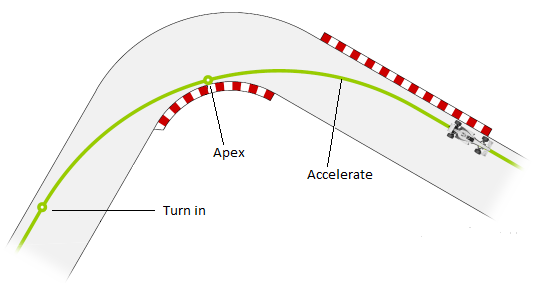
\includegraphics[height=7cm]{images/cornerraceline}
	\caption{Race line through a 90" right corner}
	\label{fig:CornerRaceLine}
\end{figure}

After the driver manages to drive the race line at a relatively slow speed, the driver must find the limit of the car. This is the maximum speed the car can be driven while still allowing the driver to have maximum control over the car. Various studies have been carried out to define such a limit in terms of the physical properties of the car and environment around it. The most important property is the level of grip the car can achieve and sustain on track. Various factors contribute to the level of grip, most notable are the tires which the car is being driven on, as the tires are the only actual contact to the track, allowing for braking, accelerating and turning forces to be transferred to the asphalt\cite{beckman1991physics}.

Each tire has two properties which are of particular interest to a drive, the slip angle and slip ratio. The slip angle is the angle between a tire’s direction of travel and the actual direction the tire is going towards. Given both the actual direction of travel and desired direction of travel are known, it becomes trivial to calculate the angle which is done by calculating the arch of the two vectors as shown in \ref{fig:slipangle}.

\begin{figure}[!htb]
	\centering
	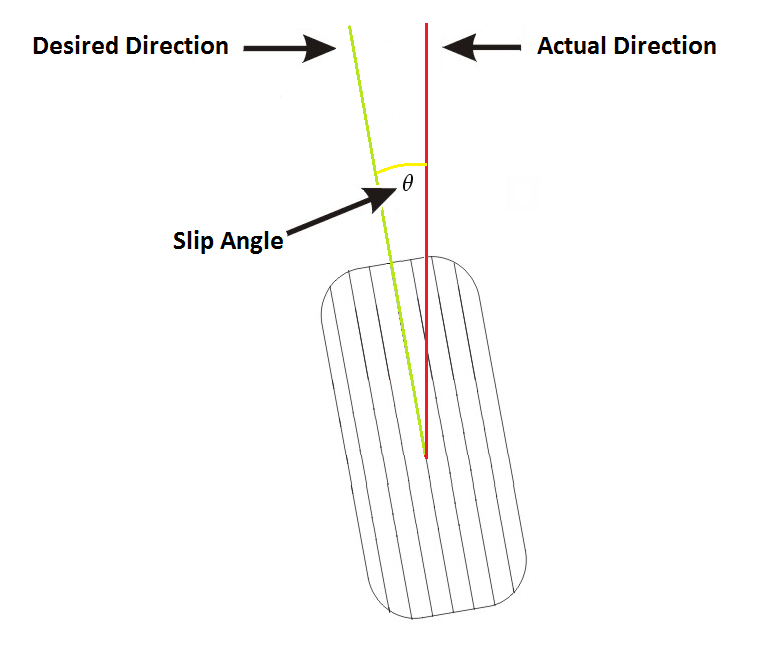
\includegraphics[height=7cm]{images/slipangle}
	\caption{Slip Angle of a tire understeering while turning left}
	\label{fig:slipangle}
\end{figure}

\subsubsection{Cornering and braking}

Whenever the slip angle is above 0’ the tire is described as being in an understeering situation. Symptoms include Light steering, drifting towards the outside of a bend and possible tyre noise from the wheels. Assuming the tires are not damaged and the track is not wet nor dirty, understeer can be caused by active factors such as cornering speed throttle, braking, steering inputs and weight transfer. Other passive factors such as Weight distribution, drive layout, suspension and chassis setup, tyre type, wear and pressures also effect understeer. An understeer situation in a corner can be avoided by not entering too fast into a corner, not accelerating too aggressively in a corner, not braking through a corner, and not making any sudden changes which drastically upset the weight distribution of the car. Passive factors have to do with the way a car is mechanically setup, such factors will be taken in consideration during this project but will not be given great importance as this project aims to improve the drive’s skills. The project will focus on the active factors as these are the ones which the driver has direct input on while driving a car. It is known for a tire to have an optimal slip angle, this is the slip angle at which the tire can produce the most grip while cornering. A common road tire’s optimal slip angle is of 5’ while a slick tire which is purpose built for racing has an optimal slip angle of 8’-10’. These values may vary a bit depending on the tire brand\cite{beckman1991physics}

Moving on to oversteer, this is an other issue which can arise from lack of grip. Whereas understeer is caused by lack of grip in the front tires, oversteer is caused by lack of grip on the rear tires. Symptoms of oversteer include having the rear of the vehicle becoming unstable and 'light' and the car starts to rotate so the driver is facing towards the inside of the corner. Active factors causing oversteer are cornering speed, throttle, braking, steering inputs and weight transfer. The driver can avoid oversteer by not braking while in a corner and not accelerating too hard in a rear wheel drive as it makes the rear tires spin too fast, losing traction with the road.

\begin{figure}[!htb]
	\centering
	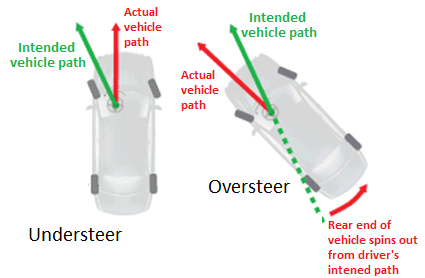
\includegraphics[height=7cm]{images/overundersteer}
	\caption{Visual representation for oversteer and understeer}
	\label{fig:slipangle}
\end{figure}

During acceleration and braking the tire experiences rotational forces, however these rotational forces do not match the expected velocity, this means at all time there is some level of slip occurring between the tire and the road beneath it. This slip is called slip ratio and is expressed in percentage. A slip percentage of 100\% would mean the tire is rotating, but the road is stationary, this is called a burnout or wheel spin. On the other hand, a percentage of -100\% would mean the tire is not rotating but the road beneath it is moving, this can occur while braking hard and is called locking the wheels\cite{pacejka2006tire}. While braking the driver must make sure not lock up the tires as this will cause the tires to wear out quicker while also drastically increasing the stopping distance. On the other hand braking too lightly will make the car take longer to decelerate with makes the driver lose time. In order to braking optimally the slip ratio should be between 10\% to 15\% \cite{GoingFaster}.

\subsection{Racing Rigs}

Moving on from the real world into the simulation world in which a racing rig is an integral part of achieving an authentic feel to the simulation experience. Racing rigs vary in price starting from a bundle with a steering wheel and pedal set costing less than €100 to ones used by professional racing teams costing thousands. The difference in price is partially due to built quality, but the biggest contributing factor is attributed to how well the rig mimics the real world. This is achieved by integrating force feedback, butt kickers and hydraulic pistons. Racing rigs can be categorised by four price range brackets. Entry level refer to the cheapest price range, racing rigs in the range offer the basics to get some one up and running.

The most basic racing rig is one which only has Steering wheel, than more sophisticated ones are made by adding pedals, shifters, racing seat, mounting frames and hydraulic pistons. Butt kickers and hydraulic pistons are commonly integrated in high end rigs such as ones built by Vesaro. Force feedback is a form of haptic technology which used to replicate the forces which are transferred through a steering wheel in a car onto the driver\cite{li2015can}. Butt kickers and hydraulic used to simulate lateral and longitudinal forces which a race driver is exposed to during racing.

\begin{figure}[!htb]
	\centering
	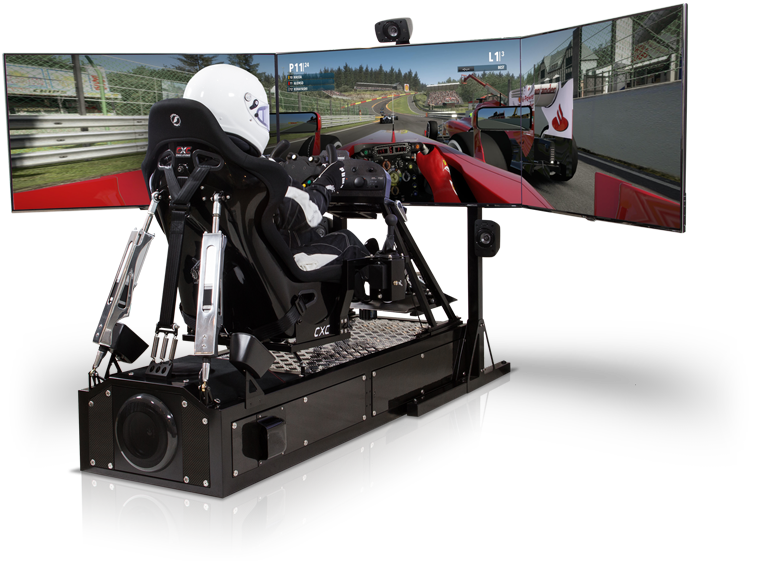
\includegraphics[height=7cm]{images/proracingrig}
	\caption{Professional racing rig by Vesaro}
	\label{fig:slipangle}
\end{figure}







